\chapter{Image Processing}
The objective is to find straight lines, image of the circumference $C$ and the image of the unknown planar curve $S$ in the provided image.

\begin{figure}[H]
    \centering
    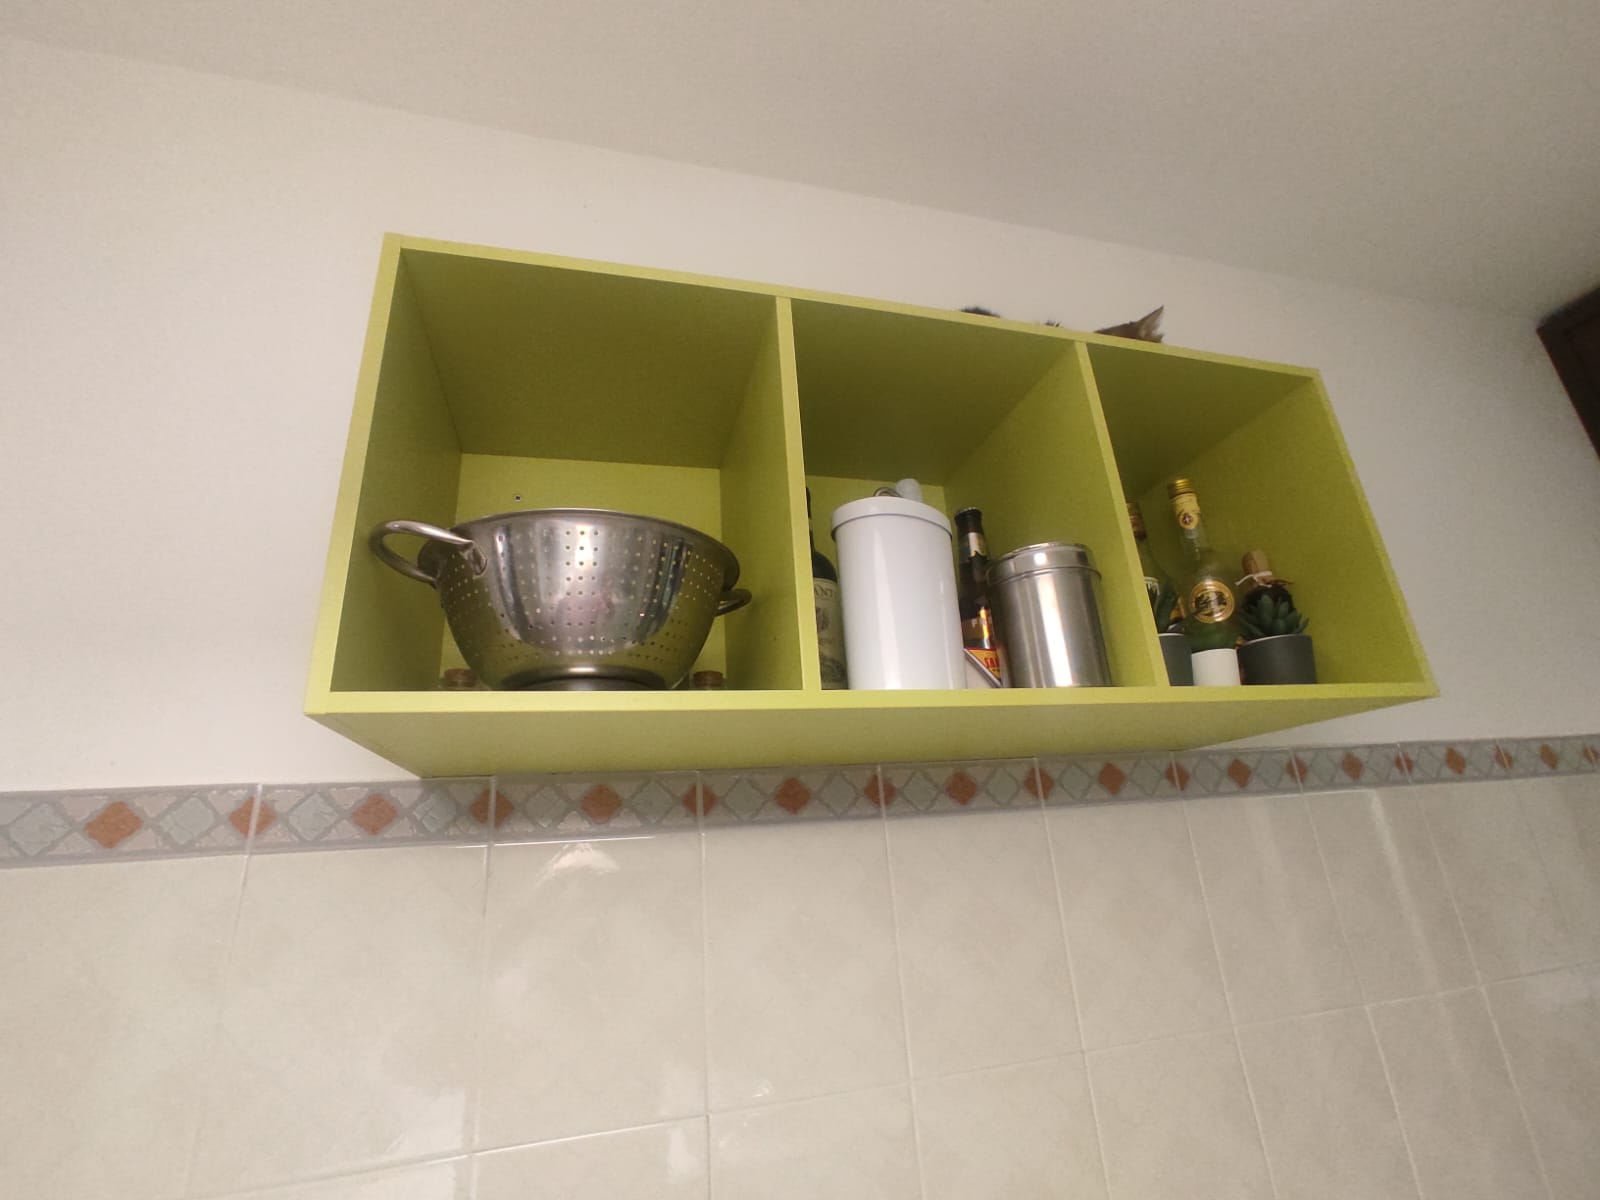
\includegraphics[width=0.75\linewidth]{img/Look-outCat.jpg}
    \caption{Original image}
    \label{fig:originalImage}
\end{figure}

\section{F1: Straight Line Detection}
The \textbf{Canny} method can be used to detect edges in the image. The algorithm works by first applying a smoothing Gaussian filter to the image (to remove noise), then computing the gradient of the image, applying nonmax suppression and tracking edges via hysteresis thresholding.
Matlab already includes (in the Image Processing Toolbox) an implementation for this method in the edge function.
First, we need to convert the image to grayscale. This way, the resulting image matrix will contain doubles in the [0,1] interval, representing the "intensity" of each pixel.

\begin{minted}{matlab}
img = im2double(imread('look-outCat.jpg'));
imgGrayscale = rgb2gray(img);
\end{minted}

Then we can simply use the edge function to apply the Canny method. A threshold can be specified to adjust the output image; in our case a value of [0.05, 0.2] seems to yield the best results.
\begin{minted}{matlab}
BW = edge(Igray, 'canny', [0.05, 0.2]);
\end{minted}

The result is pretty good, since we are able to identify some of the requested lines.
\begin{figure}[H]
    \centering
    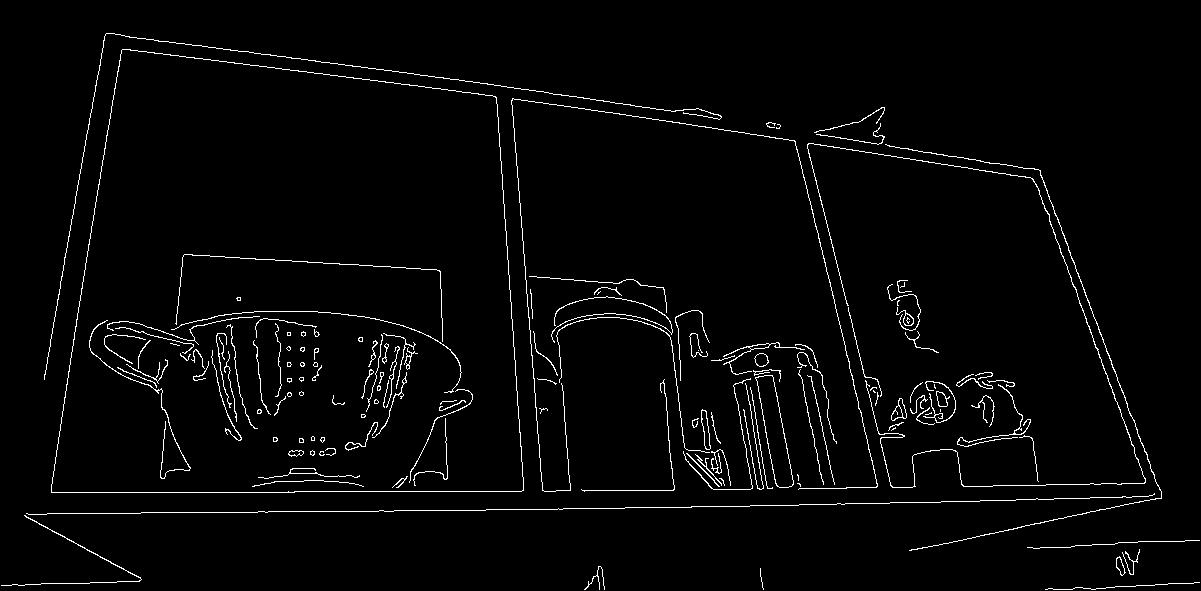
\includegraphics[width=0.75\linewidth]{img/imageProcessing/BW.jpg}
    \caption{Canny}
    \label{fig:canny}
\end{figure}

We can use the results of the previous step to detect straight lines in the image. This can be done using the \textbf{Hough transform}. A Hough transform of a datum (in this case a point on a detected edge) is a set of models compatible with the datum in the \emph{model space}.
For a point in the cartesian plane, the HT will be a sinusoid; collinear points will map to (almost) concurrent HTs.

The Hough transform is also included in Matlab:
\begin{minted}{matlab}
[H, T, R] = hough(edges);
\end{minted}
where \verb|T| is $\theta$, \verb|R| is $\rho$ and \verb|H| is a matrix whose rows and columns correspond to $\rho$ and $\theta$ values respectively.

We can then use the \verb|houghpeaks| function to detect peaks, and pass the results to \verb|houghlines| to extract lines.
\begin{minted}{matlab}
P = houghpeaks(H, 100, 'threshold', 0.3*max(H(:)));
hlines = houghlines(edges, T, R, P, 'FillGap', 4, 'MinLength', 14);
\end{minted}

These functions include various configuration options, namely:
\begin{itemize}
	\item \verb|numpeaks| is the number of peaks to detect (set to 20 here)
	\item \verb|threshold| is the minimum value to be considered a peak. By default it is set to half the maximum value in the \verb|H| matrix. For our image, we can get better results by lowering it to 30\% of the max value.
	\item \verb|FillGap| is, quoting the Matlab documentation, \emph{the distance between two line segments associated with the same Hough transform bin}. In practice, this value controls the max distance between two detected segments for them to be merged into one segment.
	\item \verb|MinLength| controls the minimum length for a segment. Setting this to a higher value allows to remove some bad segments in noisy areas of the image (e.g. the hedge).
\end{itemize}

The parameters detailed above can be adjusted based on whether we want a cleaner output or more/longer lines in the output.

\begin{figure}[H]
    \centering
    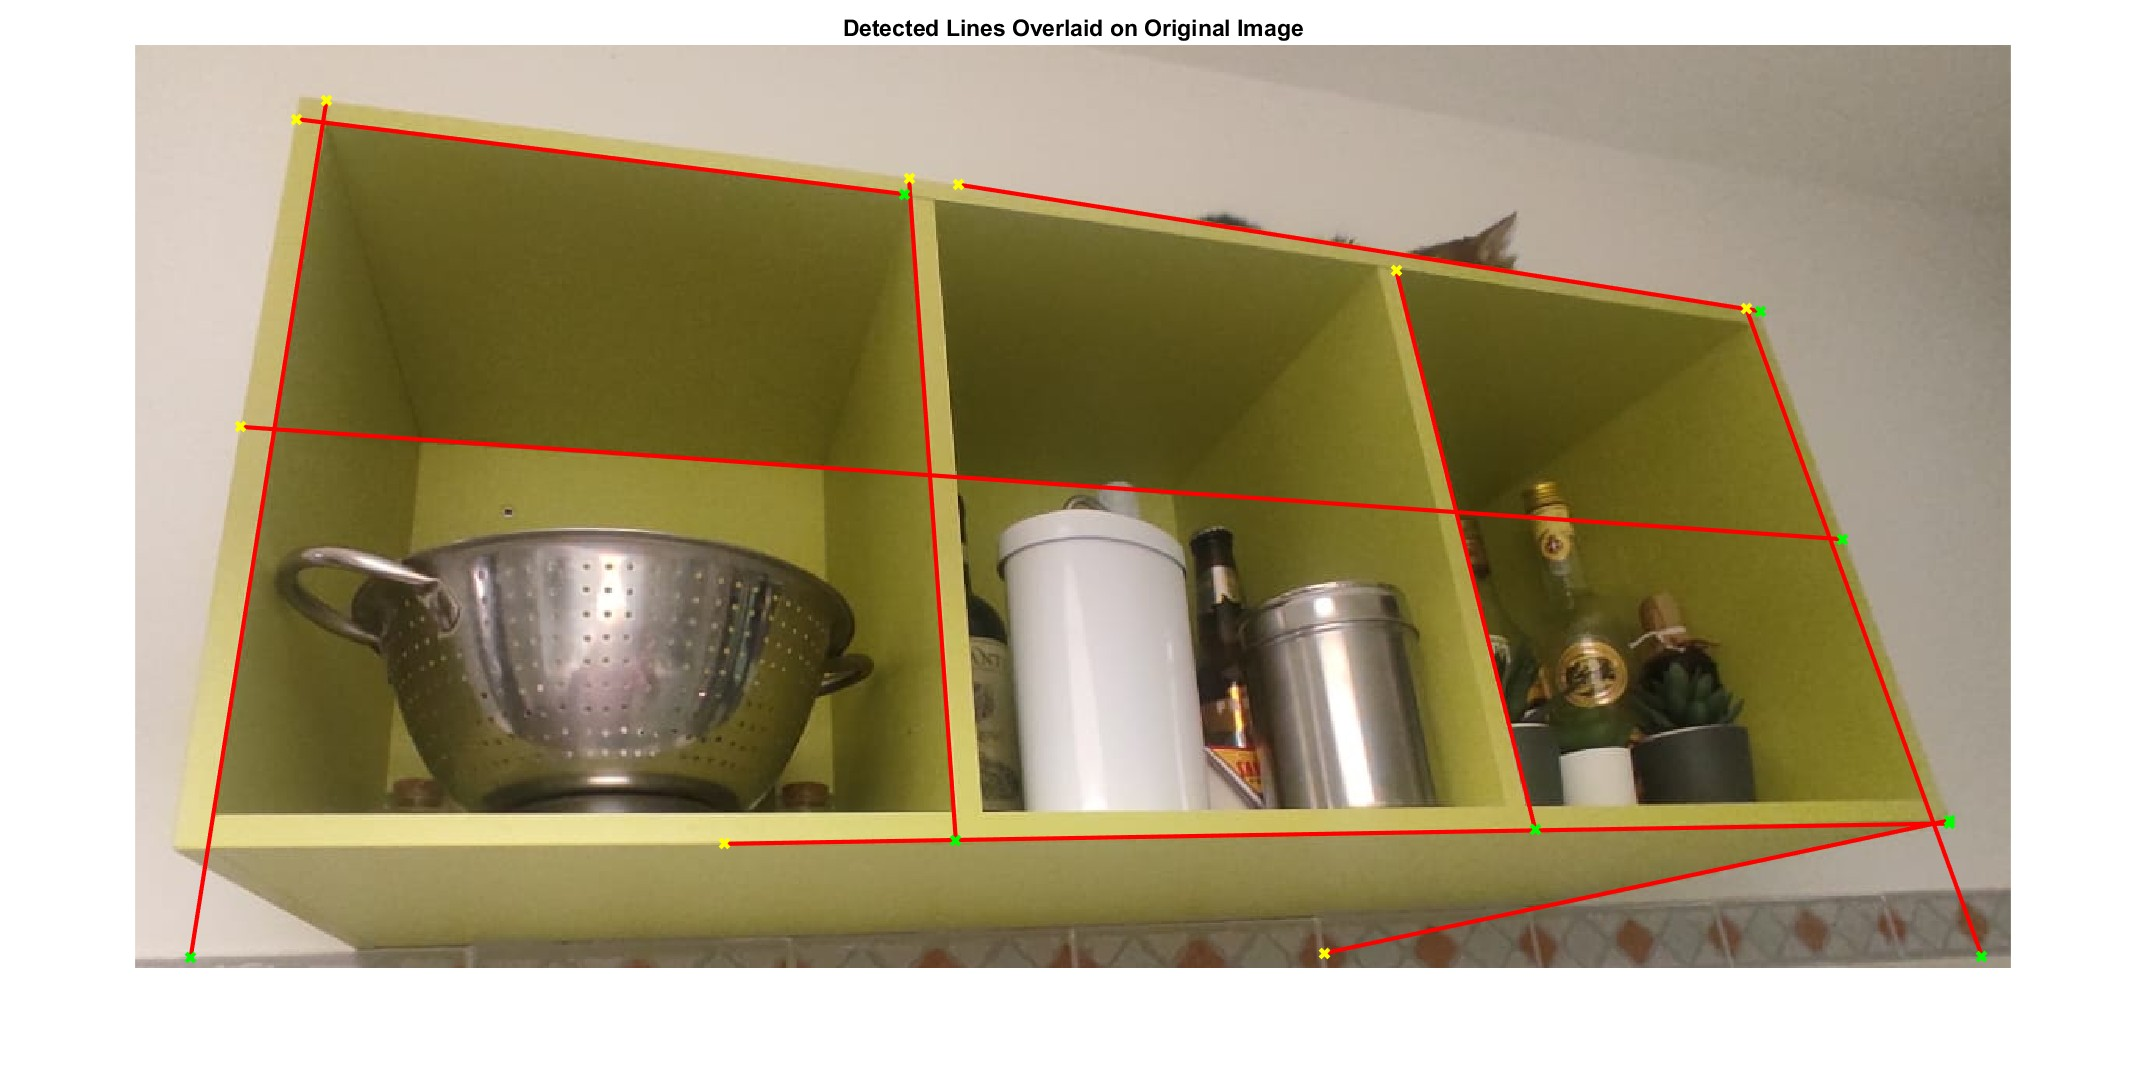
\includegraphics[width=0.75\textwidth]{img/imageProcessing/DetectedLines.jpg}
    \caption{Straight lines detected with the Hough Transform}
    \label{fig:detectStraightLines}
\end{figure}

To conclude, we were able to find precisely \verb|h| lines and some of the \verb|l| lines. The worst result is for \verb|m| lines, but increasing the contrast between dark and light areas, we could find any additional and useful edges.

\section[F2: Image of \textit{C}]{F2: Image of $C$}\label{sec:detectedC}
The goal of this task was to find the image of the circumference \verb|C| from the provided image. The task involved identifying the conic equation of the circumference based on a set of manually selected points and subsequently visualizing the computed conic on the original image.

To achieve this, the following steps were taken:

\paragraph{Point Selection:} Instead of using an interactive tool like 'getpts`, the points on the circumference were pre-defined for consistency and precision:
\begin{minted}{matlab}
   x = [417.9118, 437.6296, 456.3276, 585.1732, 721.4981, 724.8977]
   y = [566.9941, 581.6125, 526.1986, 510.9003, 543.1967, 592.1513]
\end{minted}
These points were selected manually based on the visible circumference in the image.

\paragraph{Fitting the Conic Equation:} The general conic equation is expressed as:
$$
ax^2 + bxy + cy^2 + dx + ey + f = 0
$$
To determine the coefficients $(a, b, c, d, e, f)$, a design matrix $A$ was constructed from the selected points:
$$
A = \begin{bmatrix} 
x_1^2 & x_1y_1 & y_1^2 & x_1 & y_1 & 1 \\
x_2^2 & x_2y_2 & y_2^2 & x_2 & y_2 & 1 \\
\vdots & \vdots & \vdots & \vdots & \vdots & \vdots
\end{bmatrix}
$$
The coefficients were estimated by solving $A \cdot c = 0$ using Singular Value Decomposition (SVD). The last column of the $V$ matrix from the SVD provided the solution.

\paragraph{Conic Matrix Representation:} The coefficients were used to construct the conic matrix $C$:
$$
C = \begin{bmatrix} 
a & \frac{b}{2} & \frac{d}{2} \\ 
\frac{b}{2} & c & \frac{e}{2} \\ 
\frac{d}{2} & \frac{e}{2} & f
\end{bmatrix}
$$
The matrix was normalized by dividing all elements by $C(3, 3)$.

\begin{figure}[H]
    \centering
    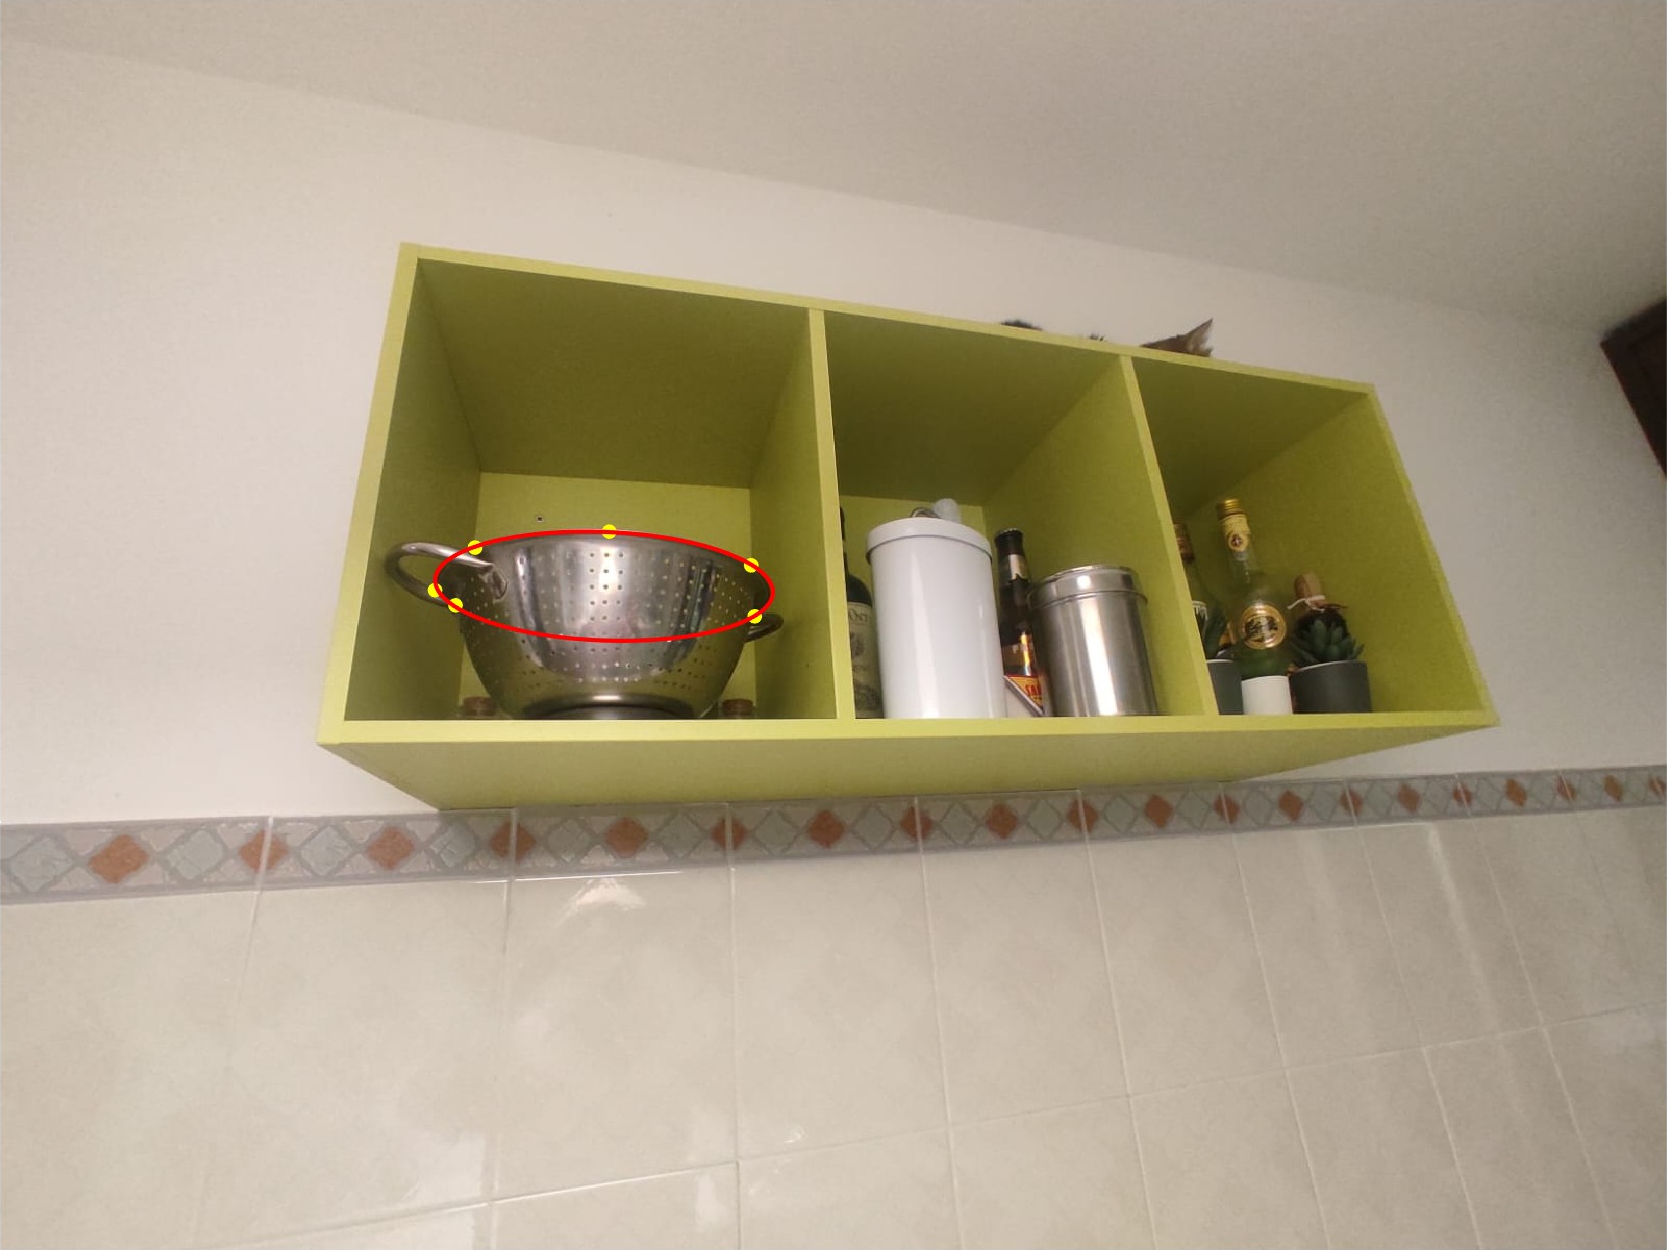
\includegraphics[width=0.75\textwidth]{img/imageProcessing/detected_conic.jpg}
    \caption{Detected conic $C$}
    \label{fig:detectedC}
\end{figure}

\section[F3: Image of \textit{S}]{F3: Image of $S$}
The goal of this task was to identify and visualize the image of a unknown curve $S$ in the provided image. This involved detecting edge points, robustly fitting an ellipse to these points using the \textbf{RANSAC} (Random Sample Consensus) algorithm, and plotting the detected curve over the original image. To focus on the elliptical curve $S$, the edge points were restricted to a predefined region of interest (ROI). This eliminated irrelevant edges outside the region containing the curve.

RANSAC was used to robustly fit an ellipse to the detected edge points in the ROI. The algorithm iteratively selects random subsets of points, fits a candidate ellipse, and identifies inliers based on their proximity to the candidate.
The best-fitting ellipse was refined by re-fitting to all inliers identified in the final RANSAC iteration.

The fitted ellipse parameters (center, axes, and orientation) were used to plot the curve $S$ as a partial ellipse. The visualization highlighted the curve on the original image, restricted to a specific segment based on its geometric properties.

The RANSAC algorithm successfully identified the elliptical curve $S$, even in the presence of noise and irrelevant edge points. The fitted ellipse was visualized as a partial curve restricted to the ROI, with endpoints refined based on geometric criteria.

I thought also to another way to solve the task, using a similar approach to what we have been used to complete the previous task, using the function \texttt{spline()} after selected manually some points on the curve.

\begin{figure}[H]
    \centering
    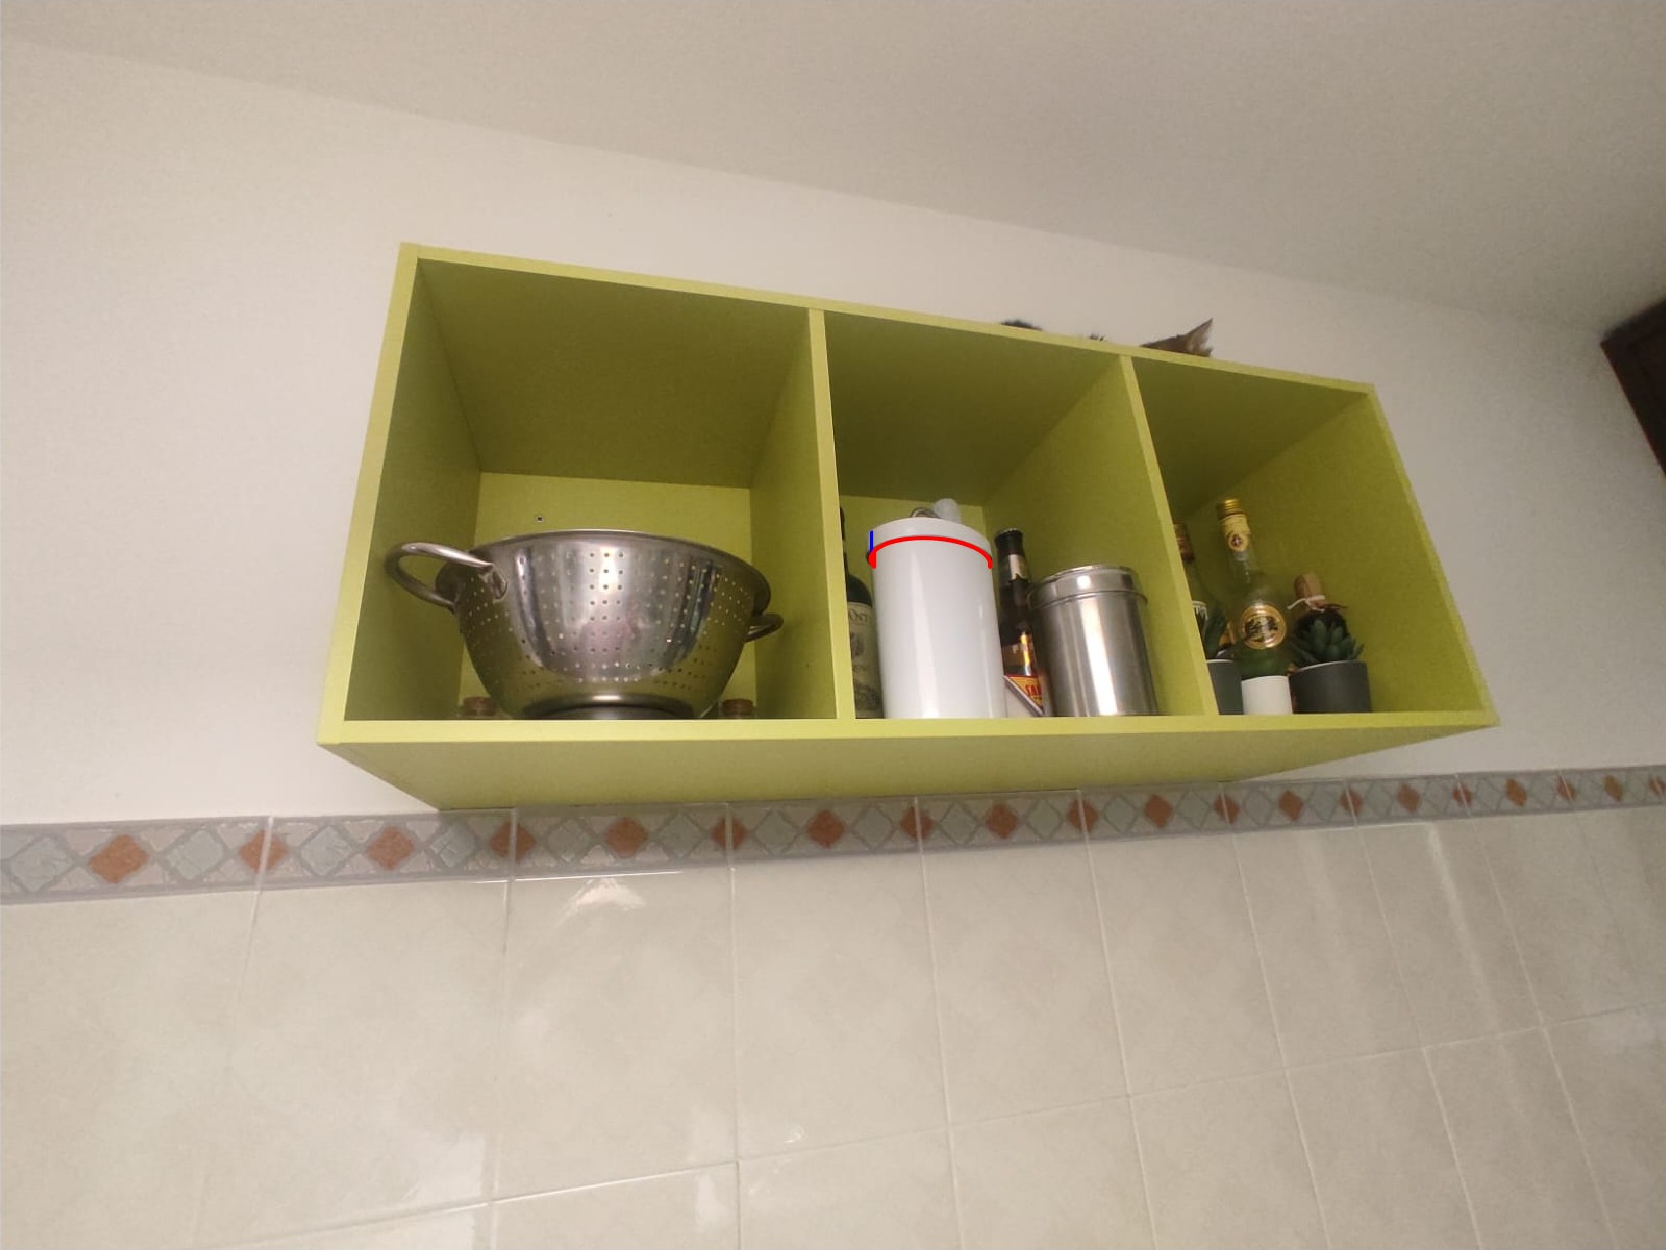
\includegraphics[width=0.75\textwidth]{img/imageProcessing/detected_s.jpg}
    \caption{Detected unknown curve $S$}
    \label{fig:detectS}
\end{figure}